\chapter{Background}
\label{chapter:RelatedWork}

Multi-task models are network architectures created with the purposes of solving multiple different but related problems in the same time. This approach yielded impressive results in many Artificial Intelligence subfields such as: Computer Vision, Natural Language Processing and Reinforcement Learning as shown in \cite{crawshaw2020multi}.

Training a model using Multi-task Learning can result in numerous benefits including faster inference and training, when compared to two or more separate networks; reduced overfitting and information optimization, as each sample becomes more valuable in a MTL environment. On the other hand, the cost of all these advantages comes in the form of the increased complexity of finding symbiotic tasks. In some scenarios, stabilizing the MT network can become a cumbersome task. This is known in the literature as \textit{negative transfer}, an unfortunate case in which learning valuable information in one task hinders the performance of one or all other tasks encapsulated in the model.

Carefully choosing tasks and formulating them in a way which benefits each other is not an exact science, which follows certain protocols, at least yet. At the moment this combination is done based on intuition and through experimentation thus reducing the negative transfer can be seen as "the art" of Multi-task models. 

There are multiple works in the literature which showcase the unreasonable effectiveness of Multi-task models, where multiple tasks "cooperate" to improve the performance in all problems tackled by the multi-headed network. Besides the increase in performance, MT has another interesting quality namely the fact that it more closely reflects human reasoning. The human learning process is almost never done in isolation, any new concept is learned through the prism of previous experiences and knowledge. Additionally, when learning multiple new concepts in the same time, the human mind usually attempts to find relationships between them. 

All this being said, the combination of multiple tasks can be achieved through multiple categories of MT architectures identified in works such as \cite{crawshaw2020multi} and \cite{zhao2023multi}. The most prevalent are the following three: cascaded, normal (parallel) and cross-talk (interactive). A schematic illustration of these can be seen in \textbf{Figure \ref{mt_net_categ}}.

\begin{figure}[htb]
    \centering
	\centerline{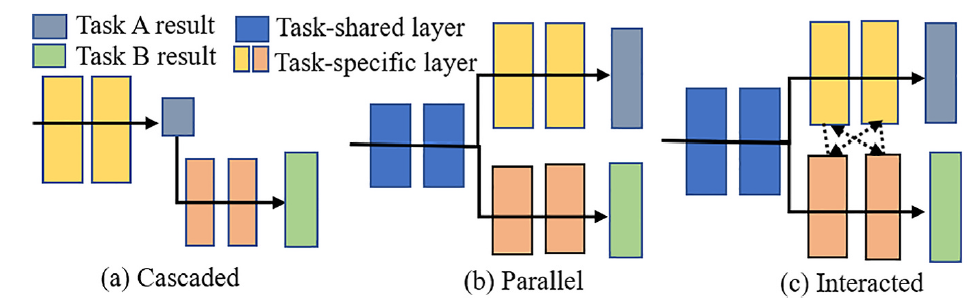
\includegraphics[scale=0.8]{figures/categories_mt_nets.png}}
	\caption{Examples of Multi-task networks classes: (a) cascaded (b) normal / parallel (c) cross-talk / interactive. Partially taken from \cite{zhao2023multi}.}
	\label{mt_net_categ}
\end{figure}

The most ubiquitous Multi-task type of network is the parallel one. In this design, a common encoder extracts valuable features which are sent in multiple independent task specific modules. Depending on the relation between the approached tasks the individual modules can be further connected via one or multiple fusion blocks in  order to further increase performance, resulting in a interacted or cross-task MT model. A cascade network is obtained when the result of one task is used as an input or feature for the remaining tasks.

Depending on the school of thought, some researchers argue that networks which process Multi-modal inputs are also included in the MT class of models. For the purposes of this report we will consider only approaches from the previously described three categories, although we will not disqualify multi-modal architectures as long as they are also part of said MT classes.

In \cite{zhao2023multi}, a vast number of medical applications of Deep Multi-task models are presented, briefly described and categorised based on their architecture and entity present in the input images. The authors showcase numerous approaches in which the MTL paradigm was used to improve performance in clinical practices which diagnose the following body areas and systems: brain, eyes, chest, cardiac, abdomen, musculoskeletal. Furthermore, they also offer a description of methods which processes histological images. 

This report differentiates itself from this impressive existing prior work through the following aspects:
\begin{itemize}
  \item The selection of papers.
  \item The perspective from which the analysis is conducted, as this report will focus on the choice of tasks (i.e. classification +  segmentation). 
  \item The granularity of the analysis especially for the papers considered to be the most representative in their category.
\end{itemize}